Le co-encadrement du stage par Rama Gottfried, qui cumule le statut de chercheur et de compositeur multimédia, a permis une réelle interaction entre informaticien et compositeur aidant à la démarche d'amélioration du logiciel \textit{symbolist}, et à la constitution de nouvelles fonctionnalités. Au-delà du développement logiciel, la conception de fonctionnalités pour \textit{symbolist} a également conduit à une réflexion sur des thématiques de recherche liées à la notation musicale.
Aussi, les aspects discutés ci-après formalise les enjeux scientifiques émergeant de la recherche de nouvelles fonctionnalités pour le logiciel \textit{symbolist}.

\subsection{La partition comme pilote des paramètres du son} 
\label{subsec:partitionPiloteSon}
Une partition peut-être vue comme une suite d'instructions (d'évènements) pour exécuter une pièce musicale \cite{bosseur2005}. Contrairement aux interactions traditionnelles où la partition est décodée par l'interprète humain pour produire de la musique, dans un environnement numérique, la partition contrôle un ou plusieurs processus informatiques (qui deviennent à leur tour des interprètes) dans le but de produire un résultat musical (ou multimédia).
Dans \textit{symbolist}, chaque symbole de la partition est décrit par un bundle OSC (voir section \ref{sec:geneseSymbolist}), qui liste, dans un format standardisé (couples adresse-valeur), les attributs du symbole associé.
Le format OSC étant standard en informatique musicale, \textit{symbolist} en tire avantage pour pouvoir communiquer des informations contenues dans une partition à d'autres processus informatiques (application, objets, composants logiciels…), dans le but de contrôler leurs paramètres d'entrées.
Alors, la question suivante se pose: comment lier, dans un paradigme de communication OSC, les attributs d'un symbole aux paramètres d'entrée d'un processus informatique?

Une exemple simple peut être pris pour illustré le principe de connexion entre attributs de symbole et paramètres de processus. La figure \ref{fig:linkingParameters} présente un exemple de partition créée avec \textit{symbolist} qui a pour but de contrôler la hauteur du son (en Hertz) produit par un synthétiseur.

\begin{figure}[H]
	\centering
	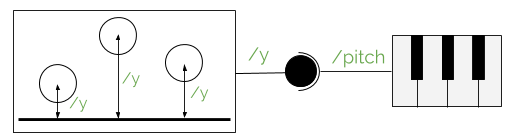
\includegraphics[keepaspectratio=true, width=\textwidth]{StructurationRecherche/i/linkingParameters.png}
	\caption{Liaison de paramètres entre une partition et un synthétiseur}
	\label{fig:linkingParameters}
	\small
	\textit{ A gauche, une partition \textit{symbolist} constitué d'un trait horizontal et d'une suite de cercles placés plus ou moins haut selon l'axe vertical. A droite, un synthétiseur, pouvant représenté un objet (au sens instance de classe), une application, ou une machine indépendante. }
\end{figure}

Dans la figure \ref{fig:linkingParameters}, le formalisme graphique utilisé pour exprimer la connexion entre les paramètres de sortie de la partition et les paramètres d'entrée du synthétiseur est celui défini par UML 2.5.1 pour modéliser les architectures de composants \cite{omg2017}. En effet, il est pratique de considérer la partition et le synthétiseur comme deux composants logiciels pour étudier la connexion de leurs paramètres. Ici, le cercle noir attaché à la partition modélise un paramètre de sortie (\textit{interface fournie}, le message OSC \texttt{/y}), et l'arc de cercle attaché au synthétiseur représente un paramètre d'entrée (\textit{interface requise}, le message OSC \texttt{/pitch}).
Dans notre exemple, le synthétiseur a besoin de l'information \texttt{/pitch}, qui représente la hauteur du son à produire en Hertz, pour pouvoir fonctionner.
De fait, connecter le paramètre \texttt{/pitch} du synthétiseur au message \texttt{/y} envoyé par la partition lie les deux valeurs selon l'expression: $/pitch = f(/y(t))$
Soit, la hauteur du son produit par le synthétiseur est une fonction de la hauteur des cercles sur l'axe vertical évoluant en fil du temps. Cette connexion peut être effectuée de deux manières: 
\begin{enumerate}[label={(\arabic*)}]
	\item \textbf{Manuellement}: l'utilisateur devra alors connaître les paramètres d'entrée du synthétiseur et envoyé les messages correspondant en sortie lors de la lecture de la partition. Dans notre exemple, l'utilisateur devra explicitement créé un message \texttt{/pitch} pour chaque cercle de la partition et l'envoyer au synthétiseur.
	\item \textbf{(Semi-)Automatiquement}: Un protocole de communication peut être mis en place pour la connexion de \textit{symbolist} et du synthétiseur; le protocole mettra en relation les messages exposés par la partition \textit{symbolist} et les messages pouvant être reçus par le synthétiseur. Aussi, l'utilisateur devra s'assurer que les paramètres sont correctement liés, d'où le caractère semi-automatique de cette procédure. 
\end{enumerate}
%
Dans les deux cas, la fonction $f$ qui permettra, pour reprendre l'exemple, de lier la valeur de \texttt{/pitch} à \texttt{/y(t)} pourra être précisée en tirant profit des expressions \textit{odot} (voir section \todo{Ajout ref expressions odot}).
Aussi, le protocole de communication devra s'assurer qu'une partition \textit{symbolist} est bien \textit{composable} avec le processus qu'elle veut contrôler. Entre autres, les interfaces exposées par l'un et l'autre doivent être compatibles \cite{chen2007}. Un des critères de la compatibilité peut simplement être la nécessité de mise en relation de paramètre du même type. Dans notre exemple, si \textit{/pitch} est de type \textit{float} et la valeur retournée par $f(/y(t))$ est une chaîne de caractères, alors la partition n'est pas composable avec le synthétiseur.

Pour réaliser cette fonctionnalité de connexion entre partition et processus de production sonore, deux technologies provenant du monde de l'informatique musicale possèdent un intérêt. La première technologie est le framework \textit{jamoma} qui permet l'encapsulation de patches Max\footnote{Pour rappel, un patch Max est une composition d'objets du langage de programmation visuelle Max. Les objets d'un patch Max sont reliés entre eux par des cordes, permettant leur communication par envoi de messages.} dans un module. Un module \textit{jamoma} déclare ses interfaces d'entrée et de sortie sous forme de liste de messages OSC, comme montré en figure \ref{fig:jamomaModule}.
\begin{figure}[H]
	\centering
	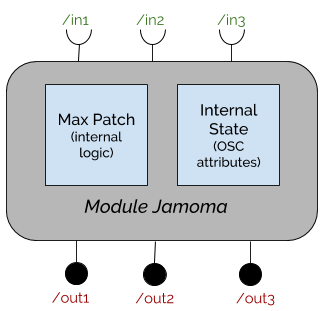
\includegraphics[keepaspectratio=true, width=0.5\textwidth]{StructurationRecherche/i/jamomaModule.png}
	\caption{Structure d'un module jamoma}
	\label{fig:jamomaModule}
	\small
	\textit{ En haut, les connexions arc de cercle représentent l'interface d'entrée du module. En bas, les connexions en cercle rempli représentent l'interface de sortie du module.}
\end{figure}
Un module \textit{jamoma} maintient un état interne (\textit{internal state} sur la figure \ref{fig:jamomaModule}) reflétant la valeur courante des attributs exposés en entrée et en sortie du module.
La connexion entre les entrées et sorties du module et le patch Max encapsulé est définie à la création du module.
L'utilisation de modules \textit{jamoma} assure une communication basée sur l'envoi de messages au format OSC, ainsi qu'une exposition explicite des messages pouvant être envoyés et reçus par un module. 

La deuxième technologie digne d'intérêt est le protocole \textit{Minuit} qui décrit un système de requêtes entre processus utilisant le format OSC comme structure interne de données \cite{minuit2010}. \textit{Minuit} définit trois types de messages pouvant être envoyés: \texttt{get} permettant de lire la valeur d'un message OSC, \texttt{set} permettant d'écrire la valeur d'un message OSC, et \textit{listen} permettant de définir un écouteur sur une valeur de message OSC. Pour reprendre l'exemple cité plus haut, le protocole \textit{Minuit} permettrait à une partition \textit{symbolist} d'écrire ou de lire la valeur de l'attribut \textit{/pitch} du synthétiseur, ou bien permettrait au synthétiseur d'être tenu au courant de la valeur courante de \texttt{/y(t)}.

\subsection{Le concept de clef}
\label{subsec:conceptDeClef}

Le concept de \textit{staff} (\gls{portee} en anglais) a été défini et implémenté dans \textit{symbolist}, précédemment au début du stage (voir section \todo{Parler plus précisément du concept de staff et ajouter un ref ici}).
Le staff est une manière d'ordonner horizontalement les symboles d'une partition \textit{symbolist} en considérant l'axe horizontal de la fenêtre graphique comme un axe temporel (dont l'extrémité gauche correspond à $t = 0$). Le staff est aussi une manière de regrouper les symboles sans pour autant enlever leur caractère individuel à chaque symbole du groupe (contrairement à la composition d'un nouveau symbole par groupement).
De fait, après avoir défini la sémantique du placement des symboles sur l'axe horizontal, la recherche de nouvelles fonctionnalités pour \textit{symbolist} a conduit à une réflexion sur la définition de la sémantique de l'axe vertical.
La CWMN (Common Western Music Notation) possède le concept de \textit{clef}, qui est un symbole placé au début d'une portée, associant à chaque ligne de la portée un nom de note.
Aussi, les notes portent le nom de la ligne sur laquelle elles se trouvent.
La figure montre un exemple de changement de clef sur une même portée qui a pour conséquence de changer le nom des notes placées à la suite.
\begin{figure}[H]
	\centering
	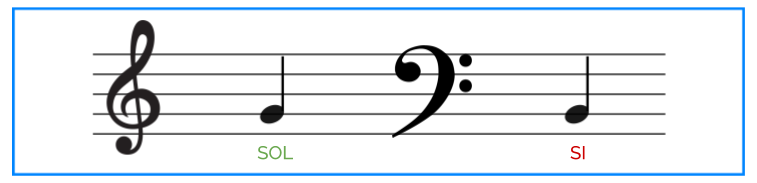
\includegraphics[keepaspectratio=true, width=0.6\textwidth]{StructurationRecherche/i/clefsCWMN.png}
	\caption{Conséquence du changement de clefs sur le nom des notes}
	\label{fig:clefsCWMN}
	\small
	\textit{A gauche, le symbole de la clef de sol suivi d'une note placée sur la deuxième ligne de la portée. A droite, le symbole de la clef de fa suivi d'une note placée sur la deuxième de la portée.}
\end{figure}
Si une clef de sol est inscrite sur la portée alors toutes les notes se trouvant à la suite sur la deuxième ligne de la portée auront pour nom \textit{sol}. Si une clef de fa est inscrite sur la portée alors toutes les notes se trouvant à la suite sur la deuxième ligne de la portée auront pour nom \textit{si}.

En s'inspirant de la CWMN, le concept de clef a été défini pour l'application \textit{symbolist}, bien qu'il ne soit pas à ce jour implémenté. 